\documentclass{article}
\usepackage{tikz}

\begin{document}

%! \usetikzlibrary{decorations.pathreplacing,decorations.pathmorphing}
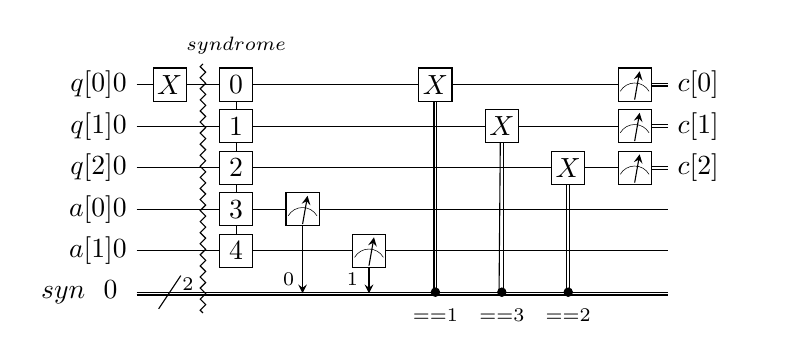
\begin{tikzpicture}[scale=1.000000,x=1pt,y=1pt]
\filldraw[color=white] (0.000000, -7.500000) rectangle (192.000000, 82.500000);
% Drawing wires
% Line 1: q0 W q[0]\ket{0} c[0]
\draw[color=black] (0.000000,75.000000) -- (180.000000,75.000000);
\draw[color=black] (180.000000,74.500000) -- (192.000000,74.500000);
\draw[color=black] (180.000000,75.500000) -- (192.000000,75.500000);
\draw[color=black] (0.000000,75.000000) node[left] {$q[0]\ket{0}$};
% Line 2: q1 W q[1]\ket{0} c[1]
\draw[color=black] (0.000000,60.000000) -- (180.000000,60.000000);
\draw[color=black] (180.000000,59.500000) -- (192.000000,59.500000);
\draw[color=black] (180.000000,60.500000) -- (192.000000,60.500000);
\draw[color=black] (0.000000,60.000000) node[left] {$q[1]\ket{0}$};
% Line 3: q2 W q[2]\ket{0} c[2]
\draw[color=black] (0.000000,45.000000) -- (180.000000,45.000000);
\draw[color=black] (180.000000,44.500000) -- (192.000000,44.500000);
\draw[color=black] (180.000000,45.500000) -- (192.000000,45.500000);
\draw[color=black] (0.000000,45.000000) node[left] {$q[2]\ket{0}$};
% Line 4: a0 W a[0]\ket{0}
\draw[color=black] (0.000000,30.000000) -- (60.000000,30.000000);
%\draw[color=black] (60.000000,29.500000) -- (192.000000,29.500000);
\draw[color=black] (60.000000,30.00000) -- (192.000000,30.00000);
\draw[color=black] (0.000000,30.000000) node[left] {$a[0]\ket{0}$};
% Line 5: a1 W a[1]\ket{0}
\draw[color=black] (0.000000,15.000000) -- (84.000000,15.000000);
%\draw[color=black] (84.000000,14.500000) -- (192.000000,14.500000);
\draw[color=black] (84.000000,15.00000) -- (192.000000,15.00000);
\draw[color=black] (0.000000,15.000000) node[left] {$a[1]\ket{0}$};
% Line 6: s W s\-0
\draw[color=black] (0.000000,0.000000) -- (192.000000,0.000000);
\draw[color=black] (0.000000,-1.000000) -- (192.000000,-1.000000);
\draw[color=black] (0.000000,0.000000) node[left] {$syn ~~0~$};
% Done with wires; drawing gates
% Line 7: s / 2
\draw (8.000000, -6.000000) -- (16.000000, 6.000000);
\draw (13.000000, 3.000000) node[right] {$\scriptstyle{2}$};
% Line 8: q0 X
\begin{scope}
\draw[fill=white] (12.000000, 75.000000) +(-45.000000:8.485281pt and 8.485281pt) -- +(45.000000:8.485281pt and 8.485281pt) -- +(135.000000:8.485281pt and 8.485281pt) -- +(225.000000:8.485281pt and 8.485281pt) -- cycle;
\clip (12.000000, 75.000000) +(-45.000000:8.485281pt and 8.485281pt) -- +(45.000000:8.485281pt and 8.485281pt) -- +(135.000000:8.485281pt and 8.485281pt) -- +(225.000000:8.485281pt and 8.485281pt) -- cycle;
\draw (12.000000, 75.000000) node {$X$};
\end{scope}
% Line 9: BARRIER
\draw[decorate,decoration={zigzag,amplitude=1pt,segment length=4}] (24.000000,-7.500000) -- (24.000000,82.500000);
% Line 10: q0 G $0$ q1 G $1$ q2 G $2$ a0 G $3$ a1 G $4$ % synd
\draw (36.000000, 82.500000) node[text width=144pt,above,text centered] {\scriptsize$syndrome$};
\draw (36.000000,75.000000) -- (36.000000,15.000000);
\begin{scope}
\draw[fill=white] (36.000000, 75.000000) +(-45.000000:8.485281pt and 8.485281pt) -- +(45.000000:8.485281pt and 8.485281pt) -- +(135.000000:8.485281pt and 8.485281pt) -- +(225.000000:8.485281pt and 8.485281pt) -- cycle;
\clip (36.000000, 75.000000) +(-45.000000:8.485281pt and 8.485281pt) -- +(45.000000:8.485281pt and 8.485281pt) -- +(135.000000:8.485281pt and 8.485281pt) -- +(225.000000:8.485281pt and 8.485281pt) -- cycle;
\draw (36.000000, 75.000000) node {$0$};
\end{scope}
\begin{scope}
\draw[fill=white] (36.000000, 60.000000) +(-45.000000:8.485281pt and 8.485281pt) -- +(45.000000:8.485281pt and 8.485281pt) -- +(135.000000:8.485281pt and 8.485281pt) -- +(225.000000:8.485281pt and 8.485281pt) -- cycle;
\clip (36.000000, 60.000000) +(-45.000000:8.485281pt and 8.485281pt) -- +(45.000000:8.485281pt and 8.485281pt) -- +(135.000000:8.485281pt and 8.485281pt) -- +(225.000000:8.485281pt and 8.485281pt) -- cycle;
\draw (36.000000, 60.000000) node {$1$};
\end{scope}
\begin{scope}
\draw[fill=white] (36.000000, 45.000000) +(-45.000000:8.485281pt and 8.485281pt) -- +(45.000000:8.485281pt and 8.485281pt) -- +(135.000000:8.485281pt and 8.485281pt) -- +(225.000000:8.485281pt and 8.485281pt) -- cycle;
\clip (36.000000, 45.000000) +(-45.000000:8.485281pt and 8.485281pt) -- +(45.000000:8.485281pt and 8.485281pt) -- +(135.000000:8.485281pt and 8.485281pt) -- +(225.000000:8.485281pt and 8.485281pt) -- cycle;
\draw (36.000000, 45.000000) node {$2$};
\end{scope}
\begin{scope}
\draw[fill=white] (36.000000, 30.000000) +(-45.000000:8.485281pt and 8.485281pt) -- +(45.000000:8.485281pt and 8.485281pt) -- +(135.000000:8.485281pt and 8.485281pt) -- +(225.000000:8.485281pt and 8.485281pt) -- cycle;
\clip (36.000000, 30.000000) +(-45.000000:8.485281pt and 8.485281pt) -- +(45.000000:8.485281pt and 8.485281pt) -- +(135.000000:8.485281pt and 8.485281pt) -- +(225.000000:8.485281pt and 8.485281pt) -- cycle;
\draw (36.000000, 30.000000) node {$3$};
\end{scope}
\begin{scope}
\draw[fill=white] (36.000000, 15.000000) +(-45.000000:8.485281pt and 8.485281pt) -- +(45.000000:8.485281pt and 8.485281pt) -- +(135.000000:8.485281pt and 8.485281pt) -- +(225.000000:8.485281pt and 8.485281pt) -- cycle;
\clip (36.000000, 15.000000) +(-45.000000:8.485281pt and 8.485281pt) -- +(45.000000:8.485281pt and 8.485281pt) -- +(135.000000:8.485281pt and 8.485281pt) -- +(225.000000:8.485281pt and 8.485281pt) -- cycle;
\draw (36.000000, 15.000000) node {$4$};
\end{scope}
% Line 11: a0:cwire +s %% 0
\draw (55.000000, 10.500000) node[text width=144pt,below,text centered] {\scriptsize $0$};
%\draw (59.500000,30.000000) -- (59.500000,0.000000);
\draw (60.00000,30.000000) -- (60.00000,0.000000);
\filldraw (60.000000, 30.000000) circle(1.500000pt);
\begin{scope}
%\draw[fill=white] (60.000000, 0.000000) circle(3.000000pt);
\clip (60.000000, 0.000000) circle(3.000000pt);
\draw (57.000000, 0.000000) -- (63.000000, 0.000000);
%\draw (60.000000, -3.000000) -- (60.000000, 3.000000);
\end{scope}
\draw[->,>=stealth] (60.000000, 10.00000)  -- +(270:10.392305pt); % arrowhead
\draw[fill=white] (54.000000, 24.000000) rectangle (66.000000, 36.000000);
\draw[very thin] (60.000000, 30.600000) arc (90:150:6.000000pt);
\draw[very thin] (60.000000, 30.600000) arc (90:30:6.000000pt);
\draw[->,>=stealth] (60.000000, 24.600000) -- +(80:10.392305pt);
% Line 12: a1:cwire +s %% 1
\draw (78.000000, 10.500000) node[text width=144pt,below,text centered] {\scriptsize $1$};
%\draw (83.500000,15.000000) -- (83.500000,0.000000);
\draw (84.00000,15.000000) -- (84.00000,0.000000);
\filldraw (84.000000, 15.000000) circle(1.500000pt);
\begin{scope}
%\draw[fill=white] (84.000000, 0.000000) circle(3.000000pt);
\clip (84.000000, 0.000000) circle(3.000000pt);
\draw (81.000000, 0.000000) -- (87.000000, 0.000000);
%\draw (84.000000, -3.000000) -- (84.000000, 3.000000);
\end{scope}
\draw[->,>=stealth] (84.000000, 10.00000)  -- +(270:10.392305pt); % arrowhead
\draw[fill=white] (78.000000, 9.000000) rectangle (90.000000, 21.000000);
\draw[very thin] (84.000000, 15.600000) arc (90:150:6.000000pt);
\draw[very thin] (84.000000, 15.600000) arc (90:30:6.000000pt);
\draw[->,>=stealth] (84.000000, 9.600000) -- +(80:10.392305pt);
% Line 13: q0 X s %% ==1
\draw (108.000000, -2.500000) node[text width=144pt,below,text centered] {\scriptsize ==1};
\draw (107.5000000,75.000000) -- (107.5000000,0.000000);
\draw (108.5000000,75.000000) -- (108.5000000,0.000000);
\begin{scope}
\draw[fill=white] (108.000000, 75.000000) +(-45.000000:8.485281pt and 8.485281pt) -- +(45.000000:8.485281pt and 8.485281pt) -- +(135.000000:8.485281pt and 8.485281pt) -- +(225.000000:8.485281pt and 8.485281pt) -- cycle;
\clip (108.000000, 75.000000) +(-45.000000:8.485281pt and 8.485281pt) -- +(45.000000:8.485281pt and 8.485281pt) -- +(135.000000:8.485281pt and 8.485281pt) -- +(225.000000:8.485281pt and 8.485281pt) -- cycle;
\draw (108.000000, 75.000000) node {$X$};
\end{scope}
\filldraw (108.000000, 0.000000) circle(1.500000pt);
% Line 14: q1 X s %% ==3
\draw (132.000000, -2.500000) node[text width=144pt,below,text centered] {\scriptsize ==3};
\draw (131.5000000,60.000000) -- (131.000000,0.000000);
\draw (132.5000000,60.000000) -- (132.5000000,0.000000);
\begin{scope}
\draw[fill=white] (132.000000, 60.000000) +(-45.000000:8.485281pt and 8.485281pt) -- +(45.000000:8.485281pt and 8.485281pt) -- +(135.000000:8.485281pt and 8.485281pt) -- +(225.000000:8.485281pt and 8.485281pt) -- cycle;
\clip (132.000000, 60.000000) +(-45.000000:8.485281pt and 8.485281pt) -- +(45.000000:8.485281pt and 8.485281pt) -- +(135.000000:8.485281pt and 8.485281pt) -- +(225.000000:8.485281pt and 8.485281pt) -- cycle;
\draw (132.000000, 60.000000) node {$X$};
\end{scope}
\filldraw (132.000000, 0.000000) circle(1.500000pt);
% Line 15: q2 X s %% ==2
\draw (156.000000, -2.500000) node[text width=144pt,below,text centered] {\scriptsize ==2};
\draw (155.5000000,45.000000) -- (155.5000000,0.000000);
\draw (156.5000000,45.000000) -- (156.5000000,0.000000);
\begin{scope}
\draw[fill=white] (156.000000, 45.000000) +(-45.000000:8.485281pt and 8.485281pt) -- +(45.000000:8.485281pt and 8.485281pt) -- +(135.000000:8.485281pt and 8.485281pt) -- +(225.000000:8.485281pt and 8.485281pt) -- cycle;
\clip (156.000000, 45.000000) +(-45.000000:8.485281pt and 8.485281pt) -- +(45.000000:8.485281pt and 8.485281pt) -- +(135.000000:8.485281pt and 8.485281pt) -- +(225.000000:8.485281pt and 8.485281pt) -- cycle;
\draw (156.000000, 45.000000) node {$X$};
\end{scope}
\filldraw (156.000000, 0.000000) circle(1.500000pt);
% Line 16: TOUCH
% Line 17: q0 M
\draw[fill=white] (174.000000, 69.000000) rectangle (186.000000, 81.000000);
\draw[very thin] (180.000000, 75.600000) arc (90:150:6.000000pt);
\draw[very thin] (180.000000, 75.600000) arc (90:30:6.000000pt);
\draw[->,>=stealth] (180.000000, 69.600000) -- +(80:10.392305pt);
% Line 18: q1 M
\draw[fill=white] (174.000000, 54.000000) rectangle (186.000000, 66.000000);
\draw[very thin] (180.000000, 60.600000) arc (90:150:6.000000pt);
\draw[very thin] (180.000000, 60.600000) arc (90:30:6.000000pt);
\draw[->,>=stealth] (180.000000, 54.600000) -- +(80:10.392305pt);
% Line 19: q2 M
\draw[fill=white] (174.000000, 39.000000) rectangle (186.000000, 51.000000);
\draw[very thin] (180.000000, 45.600000) arc (90:150:6.000000pt);
\draw[very thin] (180.000000, 45.600000) arc (90:30:6.000000pt);
\draw[->,>=stealth] (180.000000, 39.600000) -- +(80:10.392305pt);
% Done with gates; drawing ending labels
\draw[color=black] (192.000000,75.000000) node[right] {$c[0]$};
\draw[color=black] (192.000000,60.000000) node[right] {$c[1]$};
\draw[color=black] (192.000000,45.000000) node[right] {$c[2]$};
% Done with ending labels; drawing cut lines and comments
% Done with comments
\end{tikzpicture}
\end{document}
